\documentclass[12pt]{article}

%**********************************************
%* Add additional packages as needed

\usepackage{url,amsmath,setspace,amssymb,graphicx}
\usepackage{listings}

\usepackage{tcolorbox}
\usepackage{tikz}
\usepackage{xcolor}


\usepackage{color}
\def\R{\color{red}}
\def\B{\color{blue}}

\usepackage{listings}
\usepackage{caption}


%**********************************************
%* Please replace this with your name and your AAU student number
\newcommand{\studentname}{Denis D'Ambrosi}
\newcommand{\studentnumber}{12245845}



%**********************************************
%* Some more or less useful stuff, add custom stuff as needed

\lstnewenvironment{myalgorithm}[1][] %defines the algorithm listing environment
{
   % \captionsetup{labelformat=algocaption,labelsep=colon}
    \lstset{ %this is the stype
        mathescape=true,
        frame=none,
        numbers=none,
        basicstyle=\normalsize,
        keywordstyle=\color{black}\bfseries\em,
        keywords={,input, output, return, datatype, function, in, if, else, foreach, while, begin, end, },
        numbers=left,
        xleftmargin=.04\textwidth,
        #1 % this is to add specific settings to an usage of this environment (for instance, the caption and referable label)
    }
}
{}


\newtcolorbox{alert}[1]{
colback=red!5!white, colframe=red!75!white,fonttitle=\bfseries, title = #1}

\newtcolorbox{commentbox}[1]{
colback=black!5!white, colframe=black!75!white,fonttitle=\bfseries, title = #1}



%**********************************************
%* Leave the page configuration as is
\setlength{\oddsidemargin}{.25in}
\setlength{\evensidemargin}{.25in}
\setlength{\textwidth}{6.25in}
\setlength{\topmargin}{-0.4in}
\setlength{\textheight}{8.5in}

\newcommand{\heading}[5]{
\renewcommand{\thepage}{#1-\arabic{page}}
\noindent
\begin{center}
	\framebox[\textwidth]{
	\begin{minipage}{0.9\textwidth} \onehalfspacing
	{\bf 622.755 -- \unitname} \hfill #2

	{\centering \Large #5

	}\medskip
	{#3 \hfill #4}
	\end{minipage}
}
\end{center}
}

\newcommand{\unitname}{Introduction to Cybersecurity}
\newcommand{\maxpages}{5}
\newcommand{\handout}[3]{\heading{#1}{#2}{\studentname}{\studentnumber}{#3}}

%**********************************************
%* The document starts here
\begin{document}
\handout{\maxpages}{Summer Term, 2022/23}{Project Write Up}

\section{Outline}

This report investigates the implementation of Yao's protocol within the field of financial data analysis from a social, legal and ethical perspective. The paper is structured as follows: section \ref{sec:yao} introduces the protocol itself and gives an overview of my implementation of the exchange, along with a relevant use case. Section \ref{sec:applications} investigates the deployment of Yao's protocol in some areas of financial data analysis, while section \ref{sec:sel} analyzes some of social, ethical and legal questions introduced with such technology. Finally, section \ref{sec:conclusions} briefly summarizes the contents of this report.

\section{An overview of Yao's protocol}\label{sec:yao}

Yao's protocol is a two-party secure computation protocol firstly introduced by Andrew Yao in 1982 \cite{Yao82} and then re-elaborated in 1986 \cite{Yao86} that enables two parties to jointly compute a function $f$ on their private inputs $x$ and $y$ without disclosing any information about those inputs to each other. 
The protocol relies on the principle of \textit{garbled circuits}, an algorithmic technique that encodes logical circuits while mantaining their inputs secret: to execute the protocol, one party (the garbler) encrypts the circuit that computes the desired function $f$ along with its input $x$ and sends it to an evaluator who uses the encoded data to locally compute $f$ with his data $y$. This \textit{Secure Multi Party Computation} (SMPC) exchange exploits \textit{oblivious transfer}, a cryptographic procedure introduced by Rabin in an earlier paper \cite{OT} to ensure that the two parties are able to evaluate $f(x,y)$ without knowing the each other's input.

Yao's protocol offers strong privacy assurances, as neither party gains any knowledge of the other's data nor intermediate values computed during the protocol. This makes it an ideal communication primitive for applications where confidentiality is essential (see figure \ref{fig:applications}).

\begin{figure}[h]
    \centering
    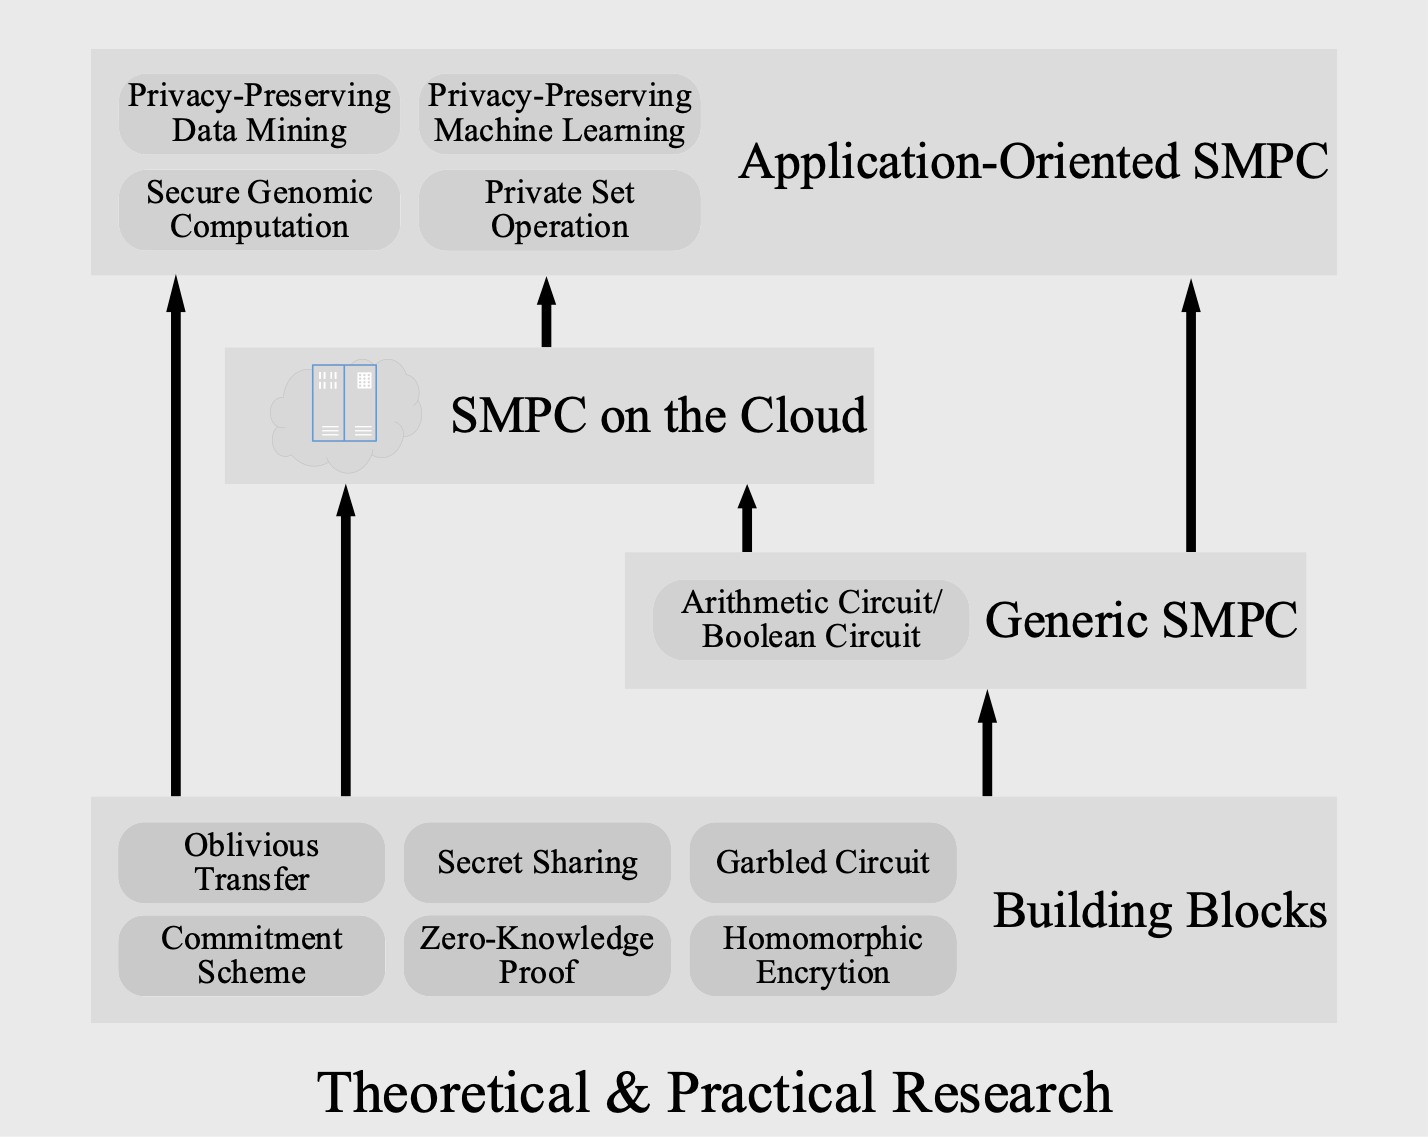
\includegraphics[width=0.6\textwidth]{practicalapplications.png}
    \caption{An overview of SMPC and its applications. Image taken from page 2 of \cite{Applications}.}\label{fig:applications}
\end{figure}

\section{Yao's protocol in the wild: how SMPC can be exploited in the financial sector}\label{sec:applications}

In the implementation part of this project, I have developed an application based on garbled circuits that allows two clients to securely compute a joint sum between their secret inputs. In financial data analysis, such functionality could be clearly beneficial to organizations that need to evaluate collective statistics without disclosing individual values. This can be especially helpful when financial institutions have to comply with strict regulatory requirements about the data involved in the computation or when the parties taking part to the exchange do not want to share secrets because of economic interests. In the remaining part of this section I will introduce some examples of actual implementations of Yao's protocol within the financial data analysis sector: needless to say, actual real-world applications calculate various functions between multiple parties, but many of them can be easily traced back to the computation of a joint sum (for example, a joint average is just a cumulative sum divided by the number of parties, which is obviously an information known in advance since the circuit must have a fixed size).

\subsection{Secure Financial Benchmarking}

The process of comparing an organization's performance against its competitors, industry standards or historical data to identify areas for improvement and set performance targets is called \textit{financial benchmarking}. Since sharing sensitive financial data with competitors and third-party benchmarking providers may clearly be the cause of several privacy concerns, by implementing a SMPC-based exchange organizations can easily compute performance metrics while easing the additional burden of ensuring data privacy.
In particular, a study by Damgard et al. \cite{Benchmarking} proposes a practical implementation of secure multi-party computation (implementing Yao's protocol) that allows banks to perform secure benchmarking for various financial metrics, like loan default rates or operational costs, without exposing sensitive information. Such protocols enable organizations to identify best practices and enhance their operations while keeping the risk of data leakage at a minimum.

\subsection{Secure Credit Scoring}

Another common process heavily (sensitive) data-dependent is \textit{secure credit scoring}: banks and other financial institutions clearly require lots of private details to assess potential borrowers before lending money away. If they exploited SMPC-based techniques instead, they would be able to compute very accurate credit evaluation of their customers without the need of disclosing personal information.

To showcase the benefits of such innovation within this field, the authors of \cite{Scoring} have proposed a secure scoring system that allows lenders to compute credit scores without directly accessing borrowers' private information through the use of SMPC. By garbling the lender's private data within the input of Yao's circuit, the user is able to evaluate his credit score locally, without sharing personal details. In this way, neither the financial institution's, nor the borrower's information are disclosed. Such approach obviously is able to guarantee customers' privacy, while alleviating concerns regarding the misuse of personal information in the process. A further upgrade to this procedure has been proposed in \cite{ScoringMining}: the authors actually show that it is possible to enhance secure credit scoring using privacy-preserving data mining techniques (for further information on this topic's state of the art refer to \cite{Mining}) to provide alternative input data sources to the credit assessment process while still respecting privacy regulations.

These secure procedures have the potential to clearly benefit all the parties involved: organizations are able to access supplementary information to compute more accurate estimates, while customers do not need to disclose private information.

\section{Ethical, Legal and Social Considerations about SMPC}\label{sec:sel}

Yao's protocol can clearly offer financial data analysis many advantages, but there are still some ethical, legal, and social concerns that must be taken into account before blindly adopting such technology. In this section, I will briefly introduce some  of the possible issues that may arise from an unresponsible use of SMPC.

\subsection{Ethical Considerations}

Even though Yao's protocol can help protecting sensitive data, it is essential that people do not let their guard down when exploiting this technique: SMPC allows for the secure computation of a shared value, but it clearly does not ensure that the choice of function, nor the inputs provided are fair and balanced. A bank could easily garble into the circuit biased input values to influence a customer's credit score and inflate his interest rates and the user would not be able to determine whether the result was tampered or not. In particular, such problems can occur when unbalanced data is input into the process: if flawled datapoints are provided by the parties to the process, the computation could easily lead to a final result that may induce discriminatory outcomes. For example, if the input data is biased towards certain demographic groups, the resulting analysis could result in investment decisions that unfairly benefit said groups.

Additionally, parties with greater resources or computing power could manipulate the protocol's outcome to their benefit, leading to unequal advantages for those in power. To address these concerns, it is essential to guarantee that the inputs provided to the protocol are representative and unbiased, with appropriate safeguards in place to prevent manipulation of its outcome.

A potential risk associated to the deployment of Yao's protocol is thus the false sense of security associated with it: this SMPC procedure can be considered truly safe only when implemented along with a set of preventive measures to control its execution.

\subsection{Legal Considerations}

Yao's protocol must also abide by the relevant data protection and privacy regulations, such as the General Data Protection Regulation (GDPR) in the European Union or California Consumer Privacy Act (CCPA) in the United States: even though the garbled-circuit exchange is inherently privacy-oriented, it is imperative to always ensure that sensitive data is managed with extreme caution. These regulations may impose specific requirements on how personal information should be handled even when encrypted to protect users' privacy and thus financial institutions must guarantee adherence to all applicable laws and regulations. For instance, a fallacious deployment of an instance of Yao's protocol could lead to the unintentional sharing of sensitive personal information such as income, investment strategies and financial goals: if customers do not give their explicit consent or the information is inadequately protected, data sharing could potentially violate said regulations.

To reduce privacy risks associated with the deployment of Yao's protocol in financial data analysis, any institution that implements it must ensure all personal data is anonymized and encrypted and appropriate consent and data security measures are in place.

\subsection{Social Considerations}

While Yao's protocol and other SMPC techniques can contribute to a societal shift towards increased data privacy and security, it is still essential to consider the potential impact on trust and transparency between the parties involved. Using SMPC in any financial process may raise concerns about data manipulation or cheating: any deviation from the agreed-upon protocols could easily lead to inaccurate or manipulated results. For example, within Yao's exchange the evaluator could easily communicate a result different from the one he locally computed and the garbler would not be able to discriminate it from an authentic outcome without additional measures into place. 

Financial institutions may thus need to establish appropriate governance structures, cryptographic verification techniques, secure computing infrastructure, and auditing procedures as well as collaborate with trusted third parties for integrity assurance in the secure computation process. By implementing these measures, one can guarantee the integrity of computation and protect against cheating by any party involved during its execution.

\section{Conclusion}\label{sec:conclusions}

After briefly introducing the dynamics of Yao's protocol, I have taken a look at some of its potential applications in financial data analysis that can allow organizations to collaborate on sensitive tasks without exposing private information. Examples such as secure financial benchmarking and credit scoring can give us a taste of its potential advantages; however, caution must still be exercised prior to implementation to ensure that deploying such secure exchanges does not introduce systematical discrimination, privacy violating mechanisms or opaqueness in the process.

{\footnotesize
\bibliographystyle{alpha}
\bibliography{references}}
\end{document}


